\section{Mockups and Wireframes}
\noindent
Based on the insights gathered during the research phase, a first version of the mockups and wireframes was designed to visualize the user interfaces and main flows.

\medskip

\noindent
The mockups were centered around the three core spaces of the platform:

\begin{itemize}
    \item \textbf{Landing Website:} Homepage presenting internship opportunities, company culture, and a call-to-action to apply.
    \begin{figure}[H]
        \centering
        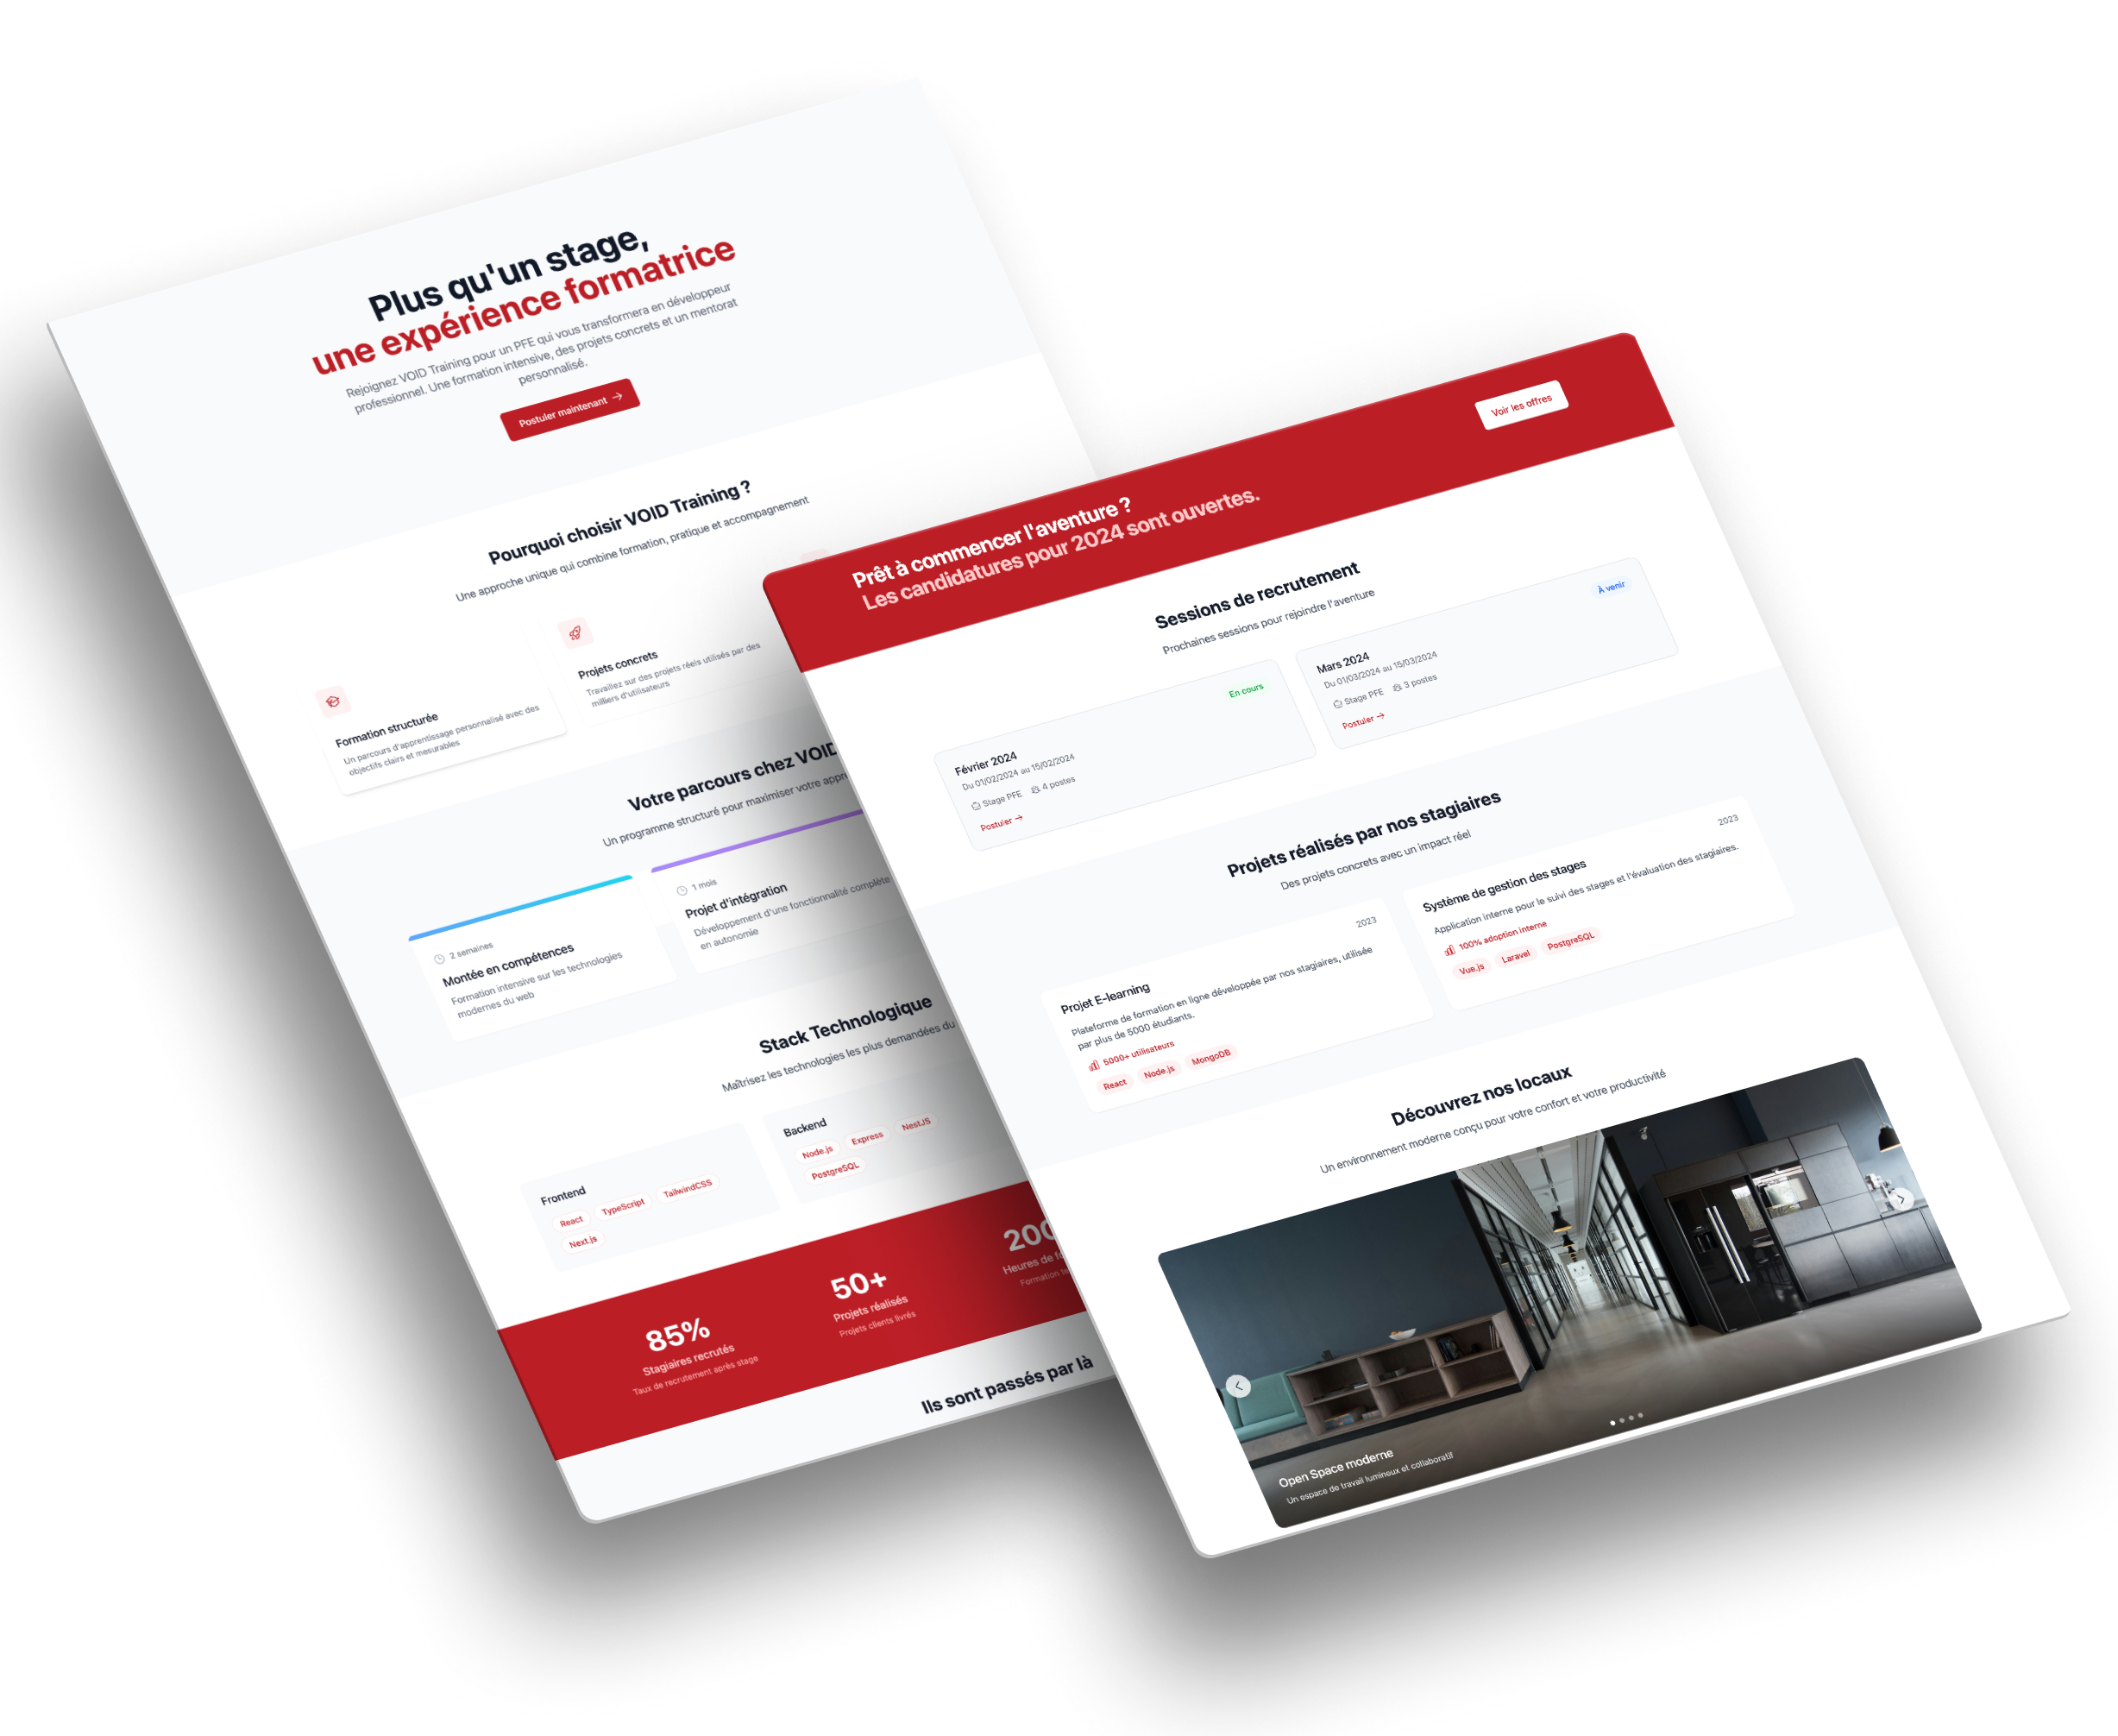
\includegraphics[width=0.\textwidth]{images/landing_mockup.png}
        \caption{High-Fidelity Mockups — Landing Website}
    \end{figure}
    \item \textbf{Candidate Space:} Area dedicated to candidates for profile creation, job application, test session participation, and training follow-up.
    \begin{figure}[H]
        \centering
        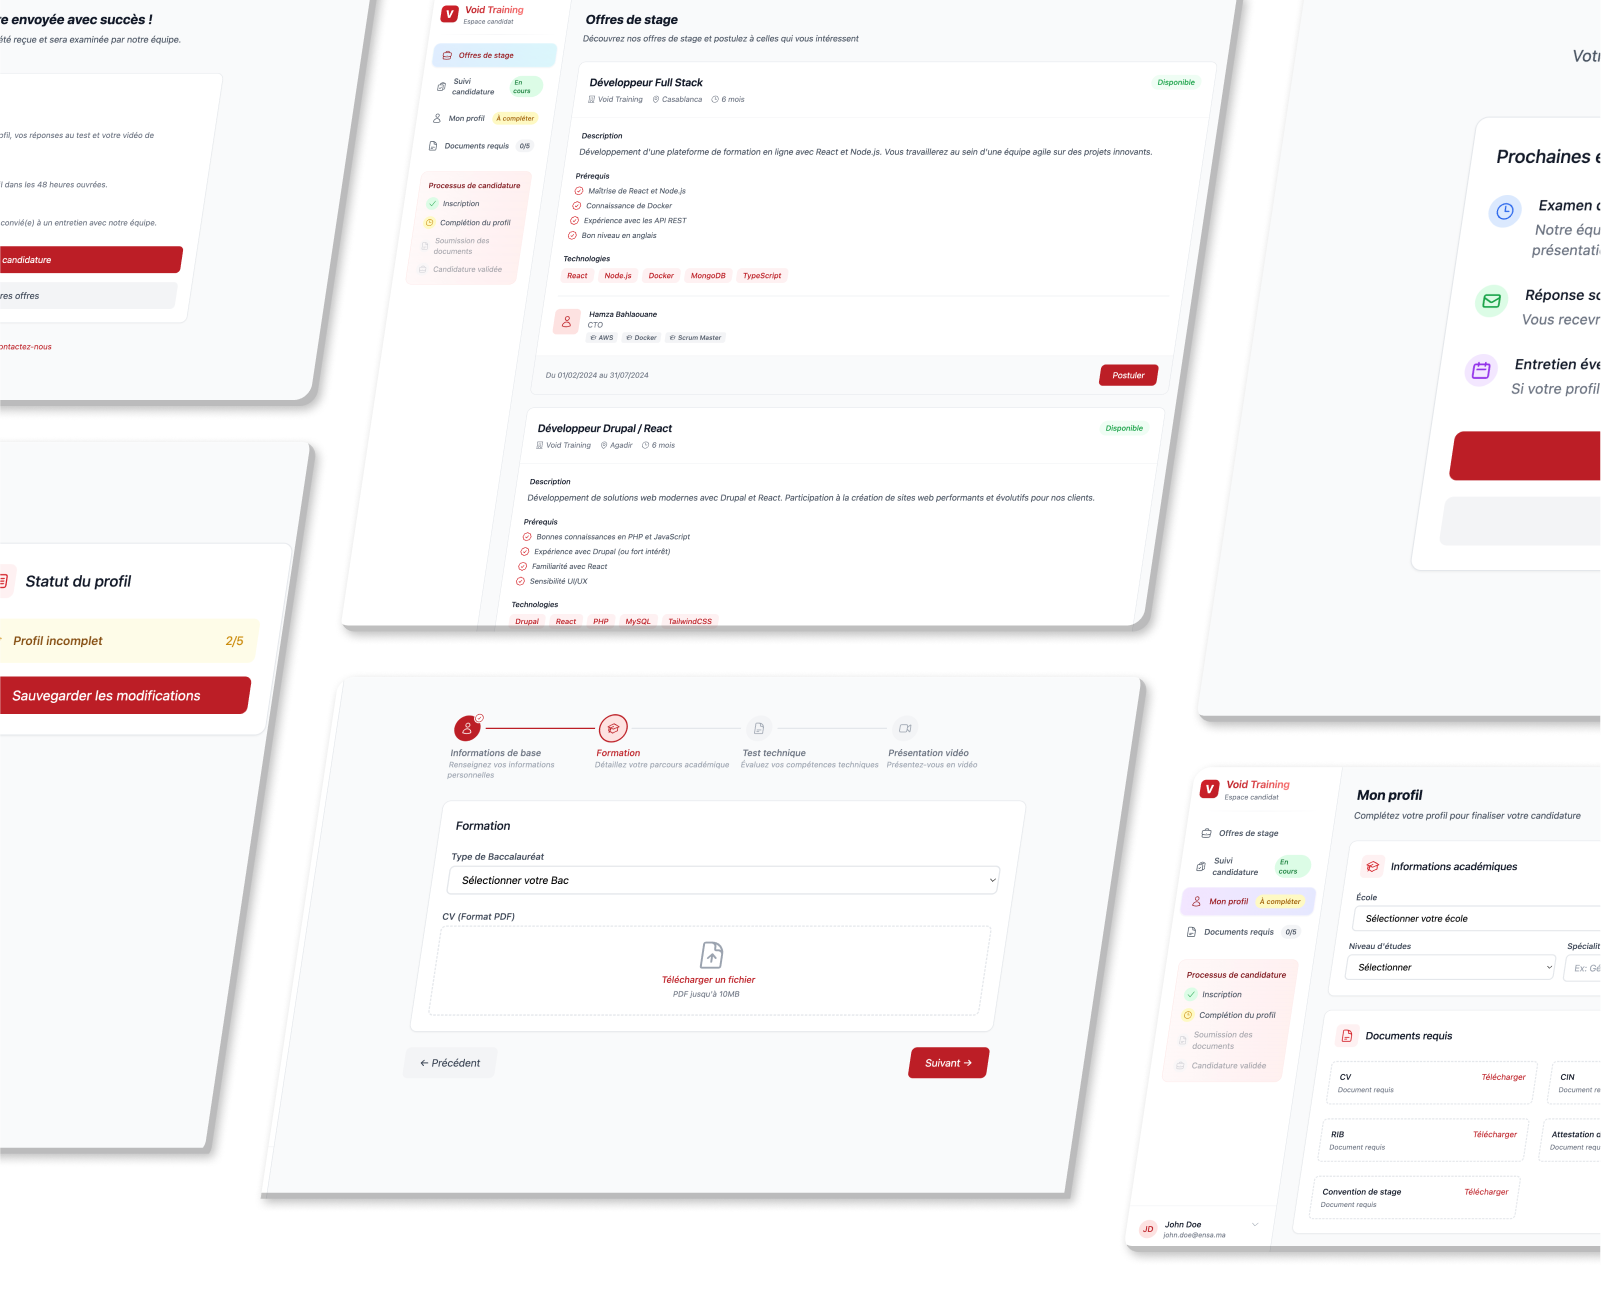
\includegraphics[width=\textwidth]{images/mockups-candidat.png}
        \caption{High-Fidelity Mockups — Candidate Space}
    \end{figure}
    \item \textbf{Training Space:} Educational portal where accepted interns can access courses, complete quizzes, and track their training progress.
    \begin{figure}[H]
        \centering
        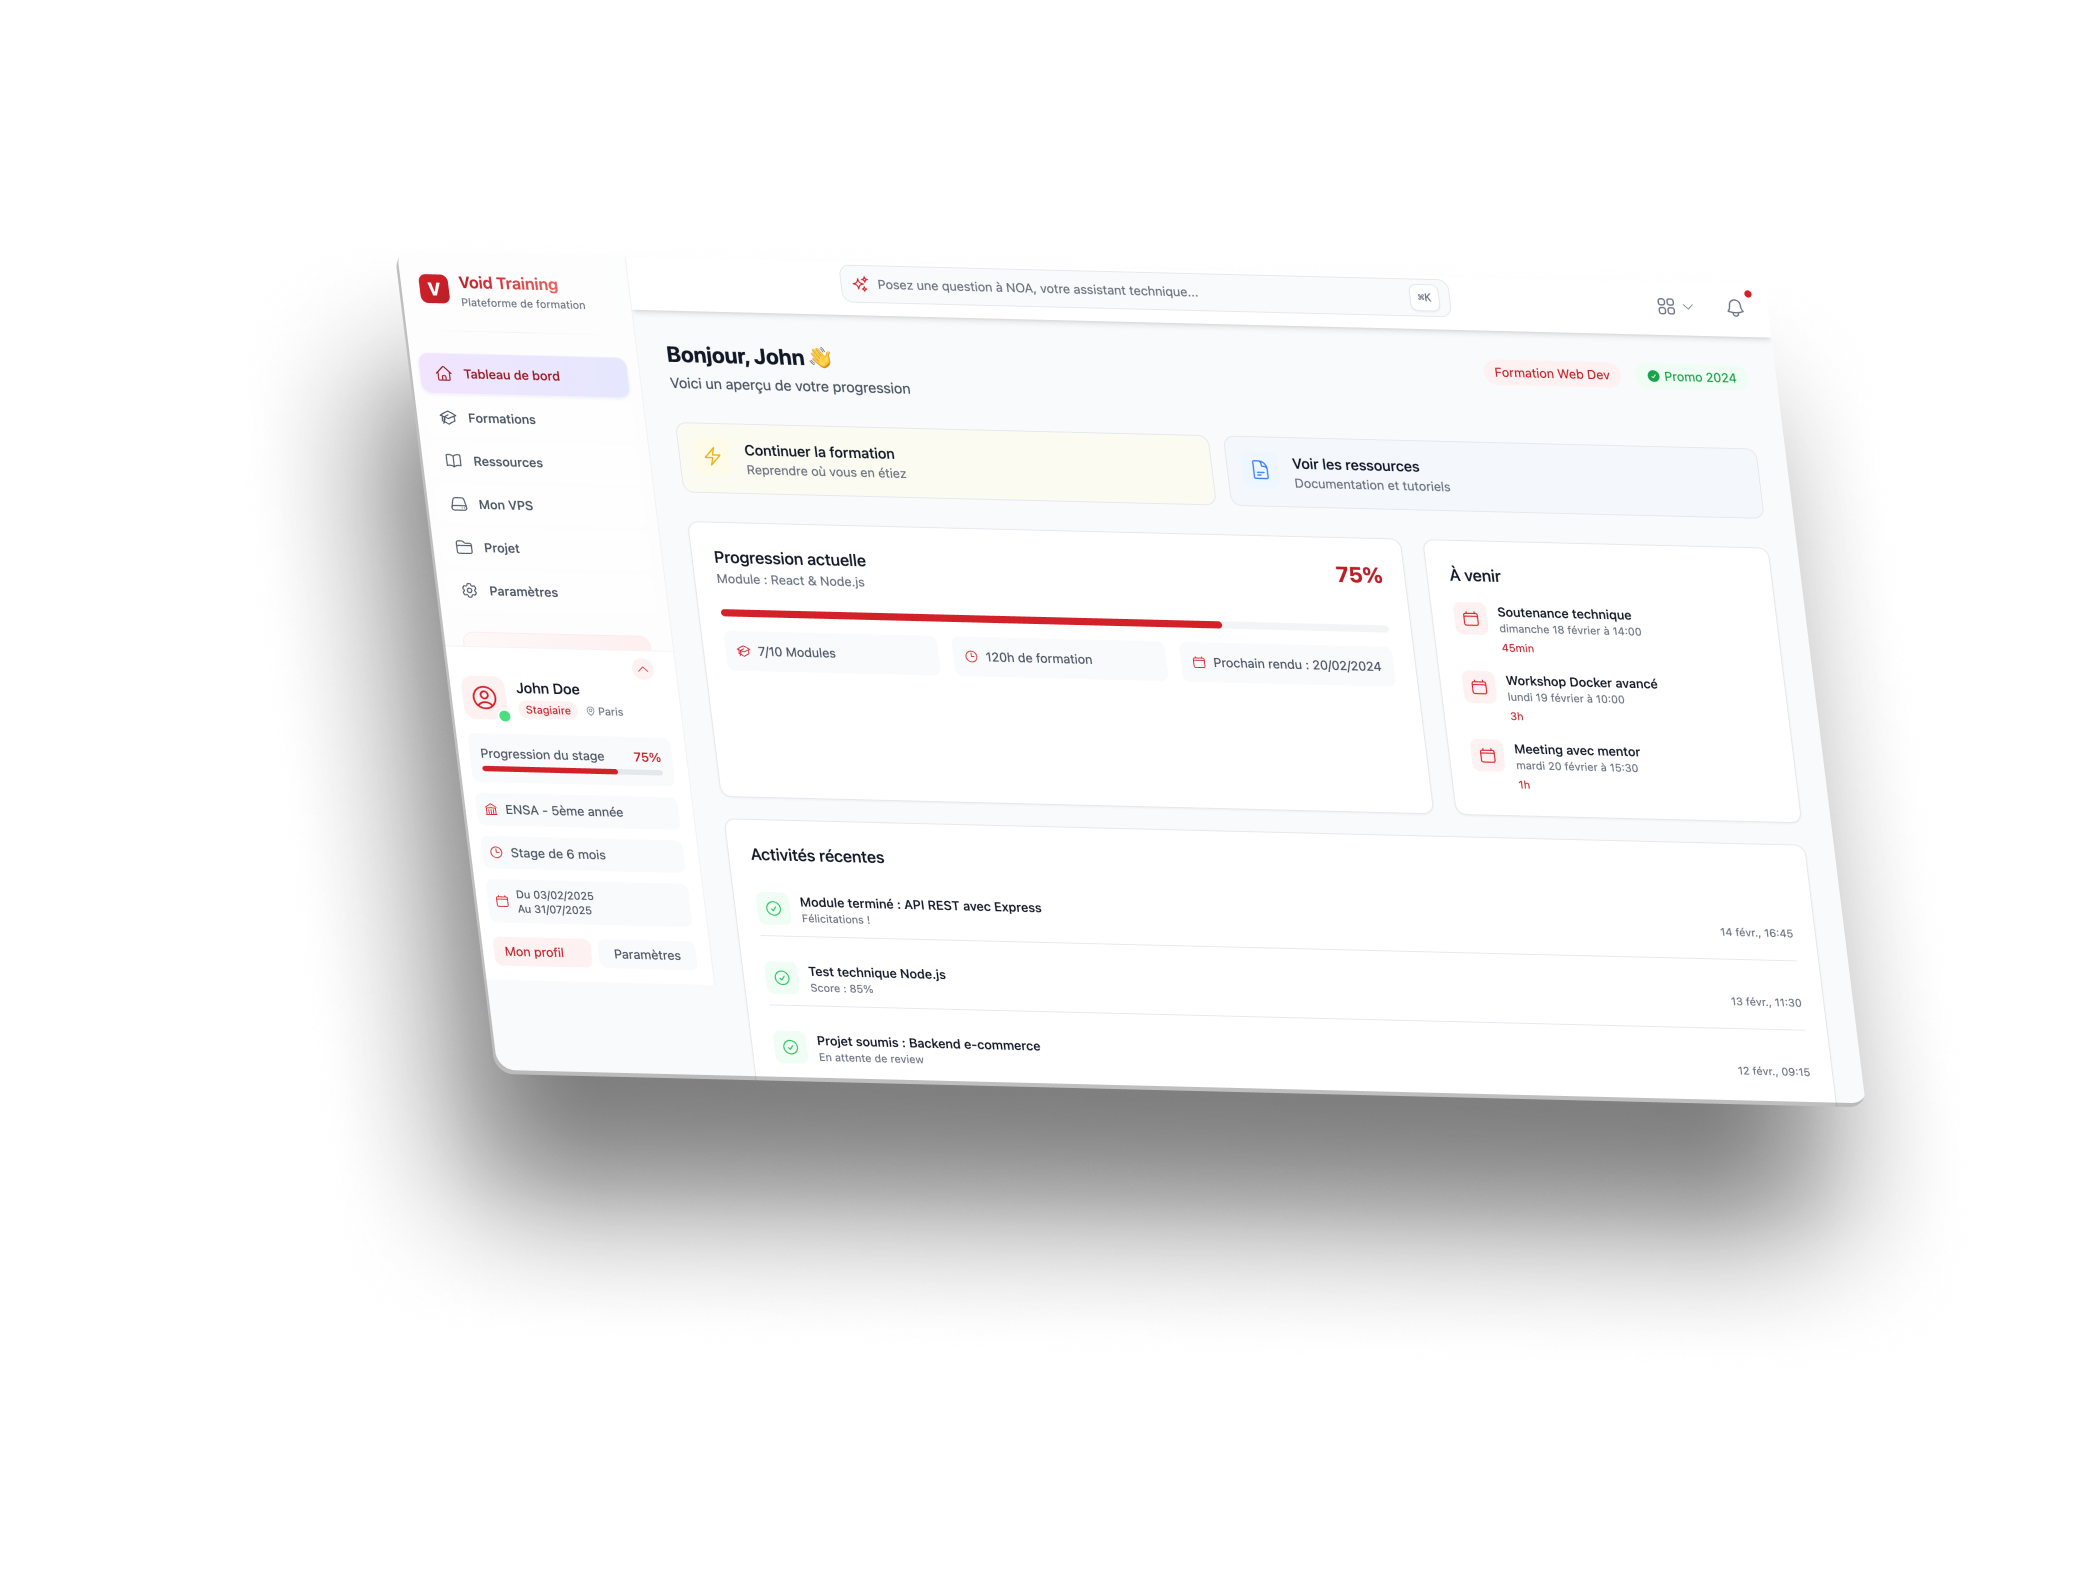
\includegraphics[width=\textwidth]{images/mockups-formation.png}
        \caption{High-Fidelity Mockups — Formation Space}
    \end{figure}
    \item \textbf{Admin Panel:} Interface for HR managers and supervisors to manage offers, monitor intern progression, and generate reports and certifications.
\end{itemize}

\medskip

\noindent
The UX design prioritized simplicity, clarity, and responsiveness to ensure a smooth experience across desktop and mobile devices.

